%!TEX root = ./main.tex

\section{The quest for a faster kNN search} % (fold)
\label{sec:the_quest_for_a_faster_knn_search}

\subsection{A short evaluation of OpenCL and CUDA} % (fold)
\label{sub:a_short_evaluation_of_opencl_and_cuda}

% subsection a_short_evaluation_of_opencl_and_cuda (end)

\subsection{Investigation of a brute force approach based on Garcia} % (fold)
\label{sub:investigation_of_a_brute_force_approach_based_on_garcia}

% subsection investigation_of_a_brute_force_approach_based_on_garcia (end)

% Possible RQ for the k-d tree section.
\begin{myrq}
\label{rq:structure_aml}
    It is possible to use a k-d tree, to increase the performance of a large number of repeated, 3-d, low k queries in a large dataset.
\end{myrq}


\subsection{Application of k-d trees to the kNN problem} % (fold)
\label{sub:application_of_kd_trees_to_the_knn_problem}

A usual strategy, when wanting to improve the performance of repeated queries in a large dataset, is to organize the dataset into some data structure especially suited for fast querying. When choosing this strategy, you are trading of the additional time penalty of building the data structure, for increased performance on each query, hopefully offsetting the build-time penalty. When considering the needs of TechnoSoft Inc, as described in section \ref{a_short_introduction_to_the_kNN_algorithm}, this strategy seems like a good fit.

In this section, we will present the k-d tree data structure, and show how it can be used for operating on three-dimensional point cloud data. Then an investigation is performed, in order to determine the possible benefits of a parallel k-d tree based algorithm.


\subsubsection{Using k-d trees for point cloud data} % (fold)
\label{ssub:using_k_d_trees_for_point_cloud_data}

A k-d tree can be thought of as a binary search tree in k dimensions. 

A few different variations exist, but we will focus our explanation around a 2D example, storing point data in all nodes. The plane is split into two sub-planes along one of the axis (in our example the y-axis) and all the nodes are sorted as to whether they belong to the left or right of this split. To determine the left and right child of the root node, the two sub-planes are again split at an arbitrary point, this time cycling to the next axis (in our example the x-axis) and the

\begin{figure}[ht!]
\centering
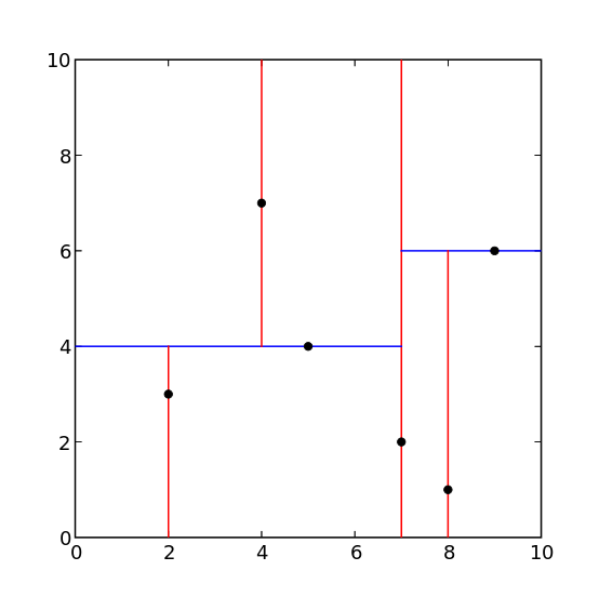
\includegraphics[width=120mm]{../gfx/Kdtree_2d.png}

\caption{2D KD-tree}
\label{fig:kdtree_2d}
\end{figure}

In order to build a k-d tree for 3D space, you simply cycle through the three dimensions, instead of two.

Given the previous splits and selection of nodes, the resulting binary tree would be as shown in the illustration under. (All illustrations gratuitously borrowed from 
%[Wikipedia](http://en.wikipedia.org/wiki/k-d_tree))

\begin{figure}[ht!]
\centering
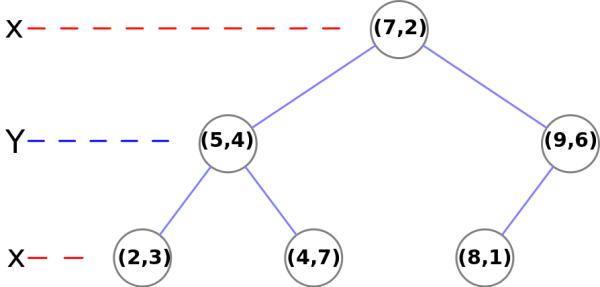
\includegraphics[width=120mm]{../gfx/Tree_0001.png}

\caption{corresponding-binary-tree}
\label{fig:tree_0001}
\end{figure}

Given that the resulting binary tree is balanced, we get an average search time for the closest neighbor in O(log2(n)) time. For values of k << n, the same average search time can be achieved, with minimal changes to the algorithm, when searching for the k closest neighbors. It is known from literature that balancing the tree can be achieved by always splitting on the meridian node. Building a k-d tree in this manner takes O(kn log2(n)) time.

Interested readers is encouraged to look at the paper Multidimensional binary search trees used for associative searching by Jon Louis Bentley, where k-d trees first was described.


% subsubsection using_k_d_trees_for_point_cloud_data (end)



\subsubsection{The serial base algorithm} % (fold)
\label{ssub:the_serial_base_algorithm}

\begin{enumerate}
    \item Build a balanced k-d tree from the point cloud.
    \item Query the tree for different sets of neighbors.
\end{enumerate}

Time complexity:

Steps:
\begin{enumerate}
    \item O(n log2 n). Achieving this speed is dependent on an efficient algorithm for finding the meridian.
    \item Approximately O(log2 n), but dependent on size of k.
\end{enumerate}

% subsection application_of_kd_trees_to_the_knn_problem (end)



\subsection{Development of a parallel kd-tree search algorithm} % (fold)
\label{sub:development_of_a_parallel_kd_tree_search_algorithm}


\section{The quest for a fast KNN search} % (fold)
\label{sec:the_quest_for_a_fast_KNN_search}

This document is a summary of our most recent (7 February 2014) findings, in the quest for a fast kNN search algorithm. The most up to date information can be found in the
%[release notes](https://github.com/hgranlund/tsi-gpgpu/tree/master/src/kNN#v14-release-notes)
for the most recent version of this project.

Our initial investigation led us to believe that a serial implementation could be as fast as the parallel brute-force solution, for point clouds with fewer than 1 000 000 points, given that both algorithms start with an unordered set of points. Reimplementing the brute-force algorithm with bitonic sort, and optimizing for three dimensions, has shown us that this initial belief was unsupported, and currently the brute force algorithm is faster when starting from a unorganized set of points. When considering repeated querying of the same point cloud, the k-d tree based solution pulls ahead, as most of its running time is spent building the k-d tree for querying. If building the k-d tree could be parallelized this could change. although documented in literature, such an parallelization is still elusive.

In order to make the document more readable, we have included short descriptions of the algorithms used, a short reference to theoretical time complexity. We then go on to list our current results, problematic areas and possible improvements.

The following papers, available in the resources folder, forms the literary basis for our current work.

Related to the brute force approach:
\begin{itemize}
    \item Improving the k-Nearest Neighbor Algorithm with CUDA - Graham Nolan
    \item Fast k Nearest Neighbor Search using GPU - Garcia et al.
    \item K-nearest neighbor search: fast gpu-based implementations and application to high-dimensional feature matching - Garcia et al.
\end{itemize}

Related to the k-d tree based approach:
\begin{itemize}
    \item Real-Time KD-Tree Construction on Graphics Hardware - Kun Zhou et al.
\end{itemize}


\subsection{Brute force based effort} % (fold)
\label{sub:brute_force_based_effort}

\subsubsection{Garcia's base algorithm} % (fold)
\label{ssub:garcias_base_algorithme}

Garcia's algorithm is based on a naive brute-force approach. It consists if two steps:
\begin{enumerate}
    \item Calculate the distance between all reference points and query points.
    \item Sort the distances and pick the k smallest distances.
\end{enumerate}

Garcias implementation supports any number of dimensions, reference points and query points (or up to ~65000, number of blocks in the GPU). Due to this feature the algorithm use a lot of extra computation power when only one query point and a small dimensions is selected.

Time complexity:

Steps:

\begin{enumerate}
    \item O(n). Every reference point must be evaluated once. Since all calculations are independent, we have a large potential for parallelizing.
    \item Insertion sort: O(pow(n, 2)).
\end{enumerate}
% subsubsection garcias_base_algorithme (end)

\subsubsection{Our reimplementation} % (fold)
\label{ssub:our_reimplementation_2}

Bitonic-sort:

Graham Nolan discusses the possibility of improving Garcia's algorithm by reimplementing step two with a bitonic sort. His source code has not been available to us, but he states that the run-time improvements was significant. As well as choosing bitonic sort for the sorting stage of our algorithm, our implementation supports up to 15 000 000 points before memory errors occur, and we have limited the number of dimensions to three.

Time complexity:

Steps:
\begin{enumerate}
    \item O(n).
    \item Bitonic sort: worst case = O(n * log2(n)), average time ( parallel) = O(log2(n)).
\end{enumerate}

Results:

Testing the different algorithms for a range of point cloud sizes and a fixed value for k, gave the following results.

\begin{figure}[ht!]
\centering
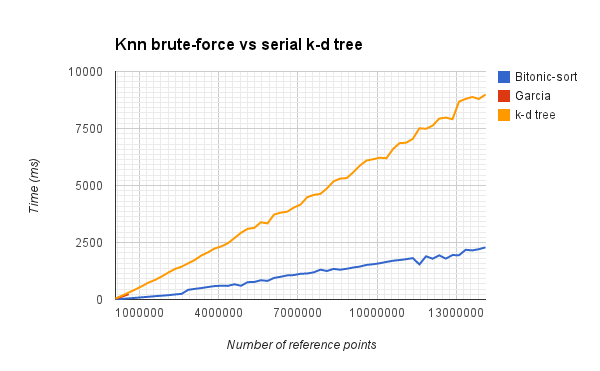
\includegraphics[width=120mm]{../gfx/knn-brute-force-vs-serial-k-d-tree.png}

\caption{knn-brute-force-vs-serial-k-d-tree.png}
\label{fig:knn_brute_force_vs_serial_k_d_tree}
\end{figure}

We see that our reimplementation of the brute-force algorithm performs well overall, notably improving on Garcia's implementation (only visible as a short line in the beginning of the graph, due to the restricted number of points it is able to compute). Still more speed is desired before good interactive usage can be achieved.

Test with n = 8 388 608:

\begin{itemize}
    \item Memory transfer 21.1 ms
    \item Calculate all distances 2.5 ms
    \item Bitonic sort 176 ms
    \item Total 200 ms
\end{itemize}

Min-Reduce:

An other possibility to improve step 2 is to use a reduce operation to get the smallest distances. This can be done k times to get the k smallest values.

Time complexity:

Steps:

\begin{enumerate}
    \item O(n).
    \item Min-reduce: k* log2(n)).
\end{enumerate}

Memory optimalisation:

We have done some memory optimization based on a
%[presentation](https://github.com/hgranlund/tsi-gpgpu/blob/master/resources/kNN/reduction.pdf)
from Nvidia.

The optimizations include:

\begin{itemize}
    \item Shared memory utilization.
    \item Sequential Addressing.
    \item Complete for-loop Unrolling.
\end{itemize}

\begin{figure}[ht!]
\centering
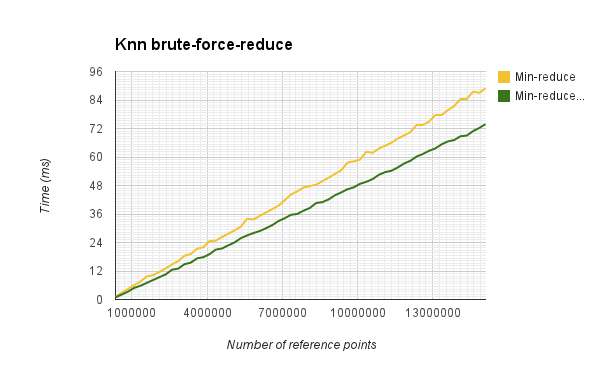
\includegraphics[width=120mm]{../gfx/knn-brute-force-reduce-memory-opt.png}

\caption{Comparison between knn-brute-force-reduce with and without memory optimizations (k=10).}
\label{fig:knn_brute_force_reduce_memory_opt}
\end{figure}

Results:

Test results of n = 8 388 608 with no memory optimization:
\begin{itemize}
    \item Memory transfer:  21.1 ms.
    \item Calculate all distances: 2.5 ms
    \item One min-reduce step : 4.8 ms.
    \item Total time: (23.7 + k*4.8) ms.
\end{itemize}

Test results of n = 8 388 608 with memory optimization:
\begin{itemize}
    \item Memory transfer:  21.1 ms.
    \item Calculate all distances: 2.5 ms
    \item One min-reduce step : 1.7 ms.
    \item Total time: (23.7 + k*1.7) ms.
\end{itemize}

\begin{figure}[ht!]
\centering
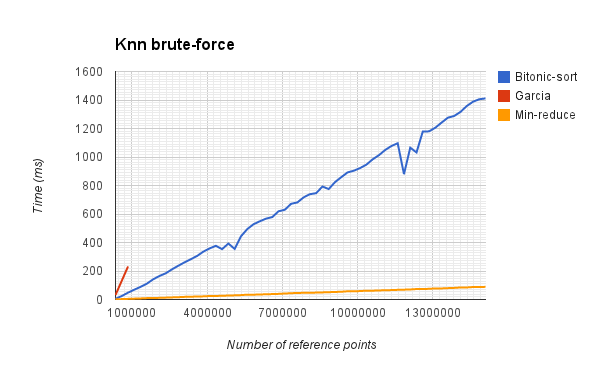
\includegraphics[width=120mm]{../gfx/BitonicVSreduce.png}

\caption{Comparison between bitonic and reduce (k=10).}
\label{fig:bitonic_vs_reduce}
\end{figure}

Possible improvements:

\begin{itemize}
    \item Memory improvements. Use shared memory and texture memory.
    \item Modify bitonic sort, so do not need to sort all points. We can split the distance array to fit into the GPU blocks, move the smallest values in each block, then sort the moved values. ~O((n/b)* b*log2(b)) subsetof O(n/b), b = Number of threads in each block, n= number of reference points
    \item Replace bitonic sort with min reduce. O(k*log2(n)).
\end{itemize}
% subsubsection our_reimplementation (end)
% subsection brute_force_based_effort (end)

\subsection{KD-tree based effort} % (fold)
\label{sub:kd_tree_based_effort}

A k-d tree can be thought of as a binary search tree for graphical data. A few different variations exist, but we will focus our explanation around a 2D example, storing point data in all nodes. The plane is split into two sub-planes along one of the axis (in our example the y-axis) and all the nodes are sorted as to whether they belong to the left or right of this split. To determine the left and right child of the root node, the two sub-planes are again split at an arbitrary point, this time cycling to the next axis (in our example the x-axis) and the

\begin{figure}[ht!]
\centering
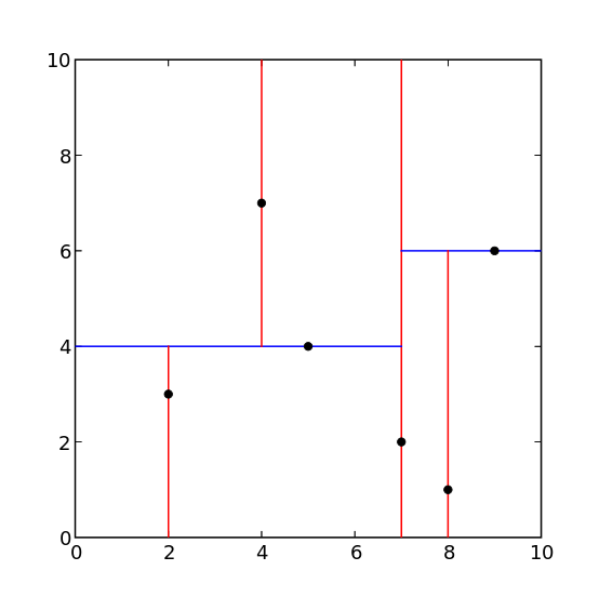
\includegraphics[width=120mm]{../gfx/Kdtree_2d.png}

\caption{2D KD-tree}
\label{fig:kdtree_2d}
\end{figure}

In order to build a k-d tree for 3D space, you simply cycle through the three dimensions, instead of two.

Given the previous splits and selection of nodes, the resulting binary tree would be as shown in the illustration under. (All illustrations gratuitously borrowed from
%[Wikipedia](http://en.wikipedia.org/wiki/k-d_tree))

\begin{figure}[ht!]
\centering
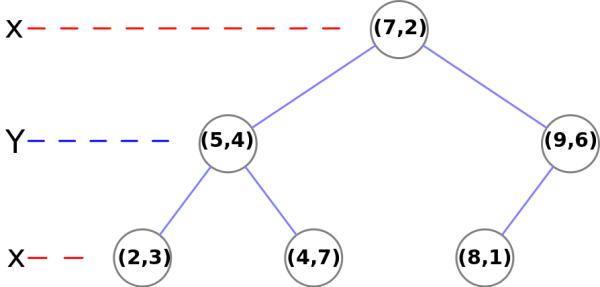
\includegraphics[width=120mm]{../gfx/Tree_0001.png}

\caption{corresponding-binary-tree}
\label{fig:tree_0001}
\end{figure}

Given that the resulting binary tree is balanced, we get an average search time for the closest neighbor in O(log2(n)) time. For values of k << n, the same average search time can be achieved, with minimal changes to the algorithm, when searching for the k closest neighbors. It is known from literature that balancing the tree can be achieved by always splitting on the meridian node. Building a k-d tree in this manner takes O(kn log2(n)) time.

Interested readers is encouraged to look at the paper Multidimensional binary search trees used for associative searching by Jon Louis Bentley, where k-d trees first was described.

\subsubsection{The serial base algorithm} % (fold)
\label{ssub:the_serial_base_algorithm}

\begin{enumerate}
    \item Build a balanced k-d tree from the point cloud.
    \item Query the tree for different sets of neighbors.
\end{enumerate}

Time complexity:

Steps:
\begin{enumerate}
    \item O(n log2 n). Achieving this speed is dependent on an efficient algorithm for finding the meridian.
    \item Approximately O(log2 n), but dependent on size of k.
\end{enumerate}

\begin{figure}[ht!]
\centering
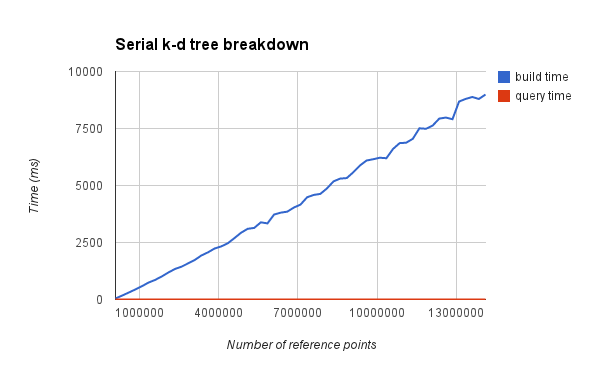
\includegraphics[width=120mm]{../gfx/serial-k-d-tree-breakdown.png}

\caption{serial-k-d-tree-breakdown}
\label{fig:serial_kd_tree_breakdown}
\end{figure}

Results:

As expected, almost all the time is spent building the tree. Querying for the closest neighbor in the largest tree took less than 0.0015 ms, but 9 seconds is a long time to wait for the tree to build.

The paper Real-Time KD-Tree Construction on Graphics Hardware - Kun Zhou et al. offers interesting, although slightly complex, ideas to an efficient parallelization of k-d tree construction. I order to save time, a good amount of time was spent searching for, and trying out, different open source implementations based on this paper. This search was unsuccessful. All the implementations we managed to find was problematic due to lack of updates, often not updated since 2011, and still running on CUDA 4.1, lack of documentation, lack of generalization or dubious source code.

A more uplifting find was several references to Real-Time KD-Tree Construction on Graphics Hardware in material published by Nvidia, regarding their proprietary systems for ray tracing. A graphics rendering technique often reliant on k-d trees, and indeed dependent on high performance.
% subsubsection the_serial_base_algorithm (end)

\subsubsection{Our reimplementation} % (fold)
\label{ssub:our_reimplementation}

Finding a way to represent the kd-tree boils down to representing a binary tree. This can be done in several ways, but we had some criteria for our representation:

\begin{itemize}
    \item The kd-tree should be memory-efficient, at best explicitly storing only the actual point coordinates. This since we want to store the largest possible amount of points on the smaller memory of the GPU.
    \item The kd-tree representation should be easy to split, distribute and join, since we want to build it on several independent processes.
\end{itemize}

After a bit of research and trial and error, we choose to represent the kd-tree as a array of structs, representing points, with an x, y and z coordinate stored in an short array. In order to turn this array into a binary tree, the following scheme was derived. Given an array, the root node of that array is the midmost element (the leftmost of the two, given an even number of elements). To find the left child of the root, you simply find the midmost element of the left sub-array, and likewise for the right child. This representation have some advantages and drawbacks.

Advantages:
\begin{itemize}
    \item Can represent binary trees where not all leaf-nodes are present. This is the minimal requirement for representing perfectly balanced k-d trees.
    \item Joining or splitting subtrees is as simple as appending or splitting arrays.
    \item Minimal memory overhead, k-d trees can even be built in-place on the array.
\end{itemize}

Drawbacks:
\begin{itemize}
    \item Cannot represent imperfectly balanced k-d trees. This mens that the median cannot be calculated through heuristic methods, but enforces a tree optimized for fast queries.
    \item Location of children and parents have to be recalculated for all basic traversing of the tree, with may reduce the performance of queries on the tree. In order to eliminate this drawback, a index cache is computed before the search is performed.
\end{itemize}

Given this representation of the kd-tree, the base kd-tree building algorithm can be expanded to the following:

Steps:
\begin{enumerate}
    \item Find the exact median (of the current split dimension) in this sub-array, and swap it to the midmost place.
    \item Go through all elements in the list, and swap elements, such that all elements lower than the median is placed to the left, and all elements higher than the median is placed to the right.
    \item Repeat for the new sub-arrays, until the entire tree is built.
\end{enumerate}

Results:

The serial kd-tree build times was similar or better than the base algorithm, so it is not discussed here

\begin{figure}[ht!]
\centering
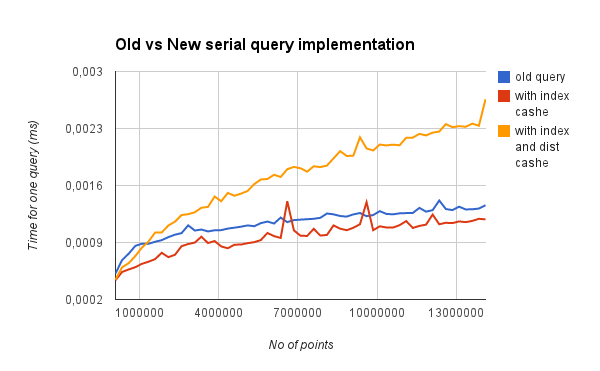
\includegraphics[width=120mm]{../gfx/awg-query-time-old-vs-new.png}

\caption{Awg query time old vs new}
\label{fig:awg_query_time_old_vs_new}
\end{figure}

The graph shows that our serial implementation of search in this data structure, given a pre-calculated index cache, is as fast, or slightly faster than the base algorithm. The possibility of improving the search even more, by storing all calculated distances in a distance cache was also explored, but we can see from the graph that the overhead associated with this operation did outweigh the benefits.

Some instability is apparent in the graph, but this is probably due to the author running other programs in the background when performing the test.

\begin{figure}[ht!]
\centering
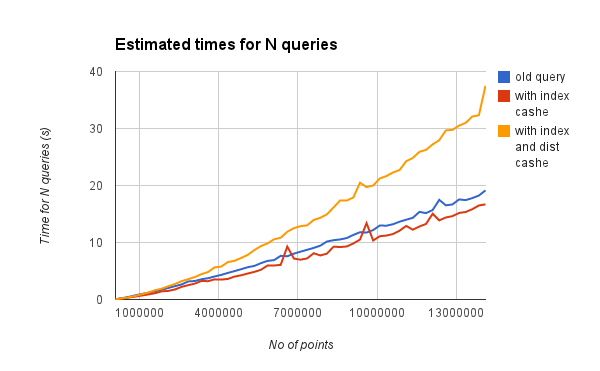
\includegraphics[width=120mm]{../gfx/n-query-time-old-vs-new.png}

\caption{n query time old vs new}
\label{fig:n_query_time_old_vs_new}
\end{figure}

The trend is exaggerated when considering N searches. Searching with an index cache is overall fastest, and gives a total search time of ~17 s for 14 million searches in a point cloud of 14 million.


Possible improvements:
\begin{itemize}
    \item Run several queries in parallel. Easy to implement, as parallelization is trivial due to independent queries, but is dependent on efficient transfer and storage of the kd-tree on the GPU.
    \item Explore performance on a variable number of k.
\end{itemize}
% subsubsection our_reimplementation (end)

\subsubsection{Parallel improvements} % (fold)
\label{ssub:parallel_improvements}

As we noted in the previous section, the kd-tree build process is by far the most expensive operation, and we would save a lot of time by managing to parallelize this operation. In order to do this, we have to look a bit closer at the different steps of the kd-tree build algorithm.

Steps:
\begin{enumerate}
    \item Find the median of the points along a specified axis. This median point becomes the value of the current node.
    \item Sort all points with lower values than the median to the left of the median, and all the points with higher values than the median to the right.
    \item Perform this algorithm recursively on the left and right set of nodes.
\end{enumerate}

Several strategies can be used to parallelize this code. We can perform the recursive calls as a increasing number of different independent processes. We can also use a parallel algorithm for finding the median in each recursive call. Both strategies can be used in conjunction with each other. The parallel algorithm for finding the median can be used to speed up the early iterations, where we do not have the possibility of calculating several sub-trees in parallel, as well as speeding up the calculation on lather calculations, by utilizing the large number of concurrent threads available in each parallel process.

Different parallel algorithms for finding the median was considered. First we tried to reuse the implementation of bitonic sort. Given a sorted list you can find the median directly, by simply looking at the midmost element of the array. Unfortunately this strategy proved unsuccessful, as re-purposing the bitonic algorithm for such an task proved difficult. We also have the inherent downside of sorting a list in order to find the median, since O(n) algorithms for finding the median exist, compared to the O(n log(n)) time required by sorting.

The existing O(n) algorithms for finding the median is mostly based on a more generic problem, namely selection or
%[kth order statistic algorithms](http://en.wikipedia.org/wiki/Selection_algorithm).
Quick select and radix select to two of the best known selection algorithms in serial. They have both an average time complexity of O(n), witch makes them a good candidates. The difference between then is the constant time penalty. The radix sort have a more exact time complexity of O(bn), where b is the number of bits in each number. While the penalty for quick select is based on n, and if bad pivot elements are chosen the worst case performance is O(pow(n, 2)). We choose to start implementing radix sort based on the results from
%[*Radix Selection Algorithm for the kth
% Order Statistic*](https://github.com/hgranlund/tsi-gpgpu/blob/master/resources/kNN/radix_select.pdf)
. Based on the constant time penalties radix sort would also be the best candidate for large number of elements (n).

The radix select is based on a bitwise partitioning, much like radix sort. In each step, elements are partitioned in two subgroups based on the current bit. Then the subgroup that contains the median is determined, and the search continue in that subgroup until the median is found.

\begin{figure}[ht!]
\centering
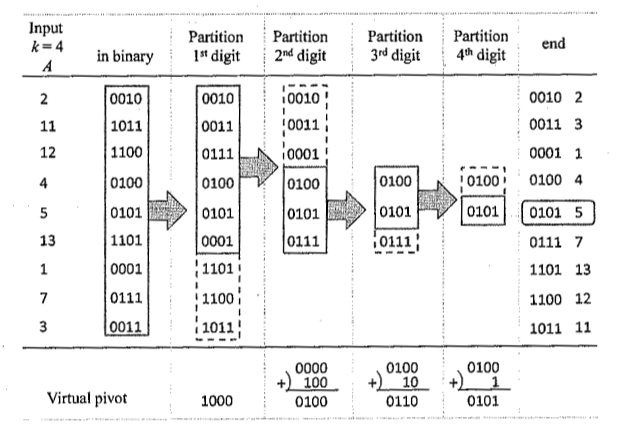
\includegraphics[width=120mm]{../gfx/Radix_select.png}

\caption{An illustration of radix selection.}
\label{fig:radix_select}
\end{figure}

It is hard to use all the parallel power of cuda in this algorithm. The reason is that the problem is divided in three different types; partition one huge list, partition some middle sized list and partition many small lists. This is the reason why we have chosen to use three different implementation of k'th order statistic. The constant time penalties of the two algorithms we have chosen give us a clear indication the radix select is best on large lists while quick select is best on small lists.

Results:
\begin{figure}[ht!]
\centering
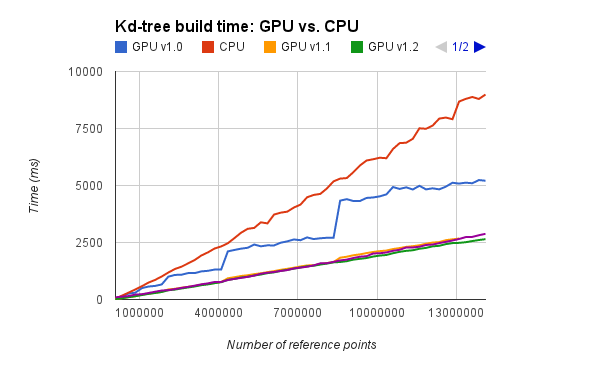
\includegraphics[width=120mm]{../gfx/gpu-vs-cpu-build-time.png}

\caption{GPU vs CPU build time.}
\label{fig:sublime_ide}
\end{figure}

We see that the parallel implementation performs better than the base serial implementation, building a tree of 14 million points in just over 5 seconds, compared to just under 10 required by the serial algorithm. Still we regard this as a quite rough implementation, in need of more tuning to really bring out the speed potential. The potential for parallelizing the workload for the first and last iterations have not been fully developed. This is due to the implementation forcing one version of the radix select algorithm being to work on all problem sizes. This is not optimal for dividing cuda resources, and as a result, we get high penalties when the problem size reaches unsuitable values.

We also see a couple of large jumps in the graph. This happens when the number of elements passes a power of two and the height of the resulting kd-tree increase. The height increase hits the implementation at its weakest.

Tuning the algorithm to alternate between radix select and quick select, eliminates this problem, as is visible in the graph for GPU v1.1. This removes the penalty for calculating the median at unsuitable problem sizes, giving an build time of ~2.4 seconds for 14 million points, compared to the ~9 seconds required by the serial implementation, or the ~5.2 seconds required by the old parallel implementation.

Memory usage:

To analyses the space complexity of the kd-tree build and search algorithm, we have made an theoretical calculation of both algorithms GPU memory consumption, and tested it against results from a GeForce 560ti and a Nvidia grid K520 (amazon web service delved).

It is important to note that the only hard memory limitation is related to building the tree, as a search for N query-points can be performed in several operations. If you e.g. run into memory limitations when searching for pow(10, 8) query-points, you can simply perform two searches on pow(5, 8) query-points to get around the limitation. Loading the pre-built kd-tree on the GPU for searching, and performing one query for a low value of k, will always consume less memory than building the actual kd-tree.

**Kd-tree-build**

The memory consumption for the kd-tree build is only depended on the number of points (n) and the theoretical consumption rate grows linearly as O(36n) subset of O(n).

\begin{figure}[ht!]
\centering
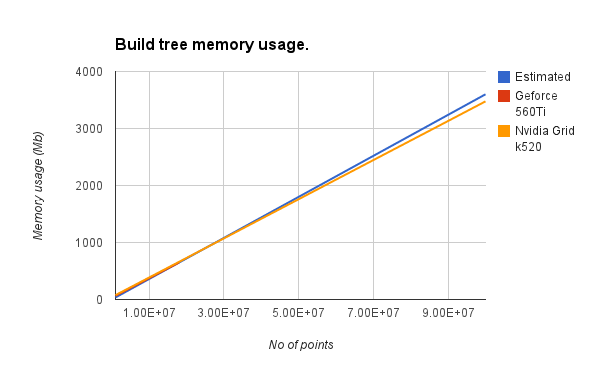
\includegraphics[width=120mm]{../gfx/memory-usage-build.png}

\caption{Memory usage of kd-tree-build.}
\label{fig:memory_usage_build}
\end{figure}

We see that the estimation fit the real consumption almost perfectly, and with this memory model, we can easily estimate the GPU memory requirements for different problem sizes.

Given that a customer wants to perform a knn-search on a point cloud of 100 million, he or she would need a GPU with at least 3.6 Gb of spare memory. Under we have tabulated what maximum problem sizes you would expect to be able to run on a selection of Nvidia graphics cards:

\begin{center}
    \begin{tabular}{ | l | l | p{5cm} |}
    \hline
    Nvidia GPU & Available memory & Maximum problem size \\ \hline
    GTX TITAN & 6144 MB & 1.79E+08 \\ \hline
    GTX 780 & 3072 MB & 8.95E+07 \\ \hline
    GTX 770 & 2048 MB & 5.97E+07 \\ \hline
    Quadro K6000 & 12288 MB & 3.58E+08 \\ \hline
    Quadro K5000 & 4096 MB & 1.19E+08 \\ \hline
    Quadro K4000 & 3072 MB & 8.95E+07 \\ \hline
    Tesla K40 & 12288 MB & 3.58E+08 \\ \hline
    Tesla K20 & 5120 MB & 1.49E+08 \\ \hline
    \end{tabular}
\end{center}

These numbers should be read as rough estimates, as each card is expected to have internal processes requiring an unspecified constant amount of the available memory, therefor lovering the maximum problem size possible to run on these cards in practice. It is also worth to mention that when buying a GPU for GPGPU tasks, other performance characteristics is equally, or more, important.

**Kd-search**

The kd-search is used to query every point against each other. It has a theoretical memory consumption rate at O((40+4k)n) subset of O(kn). The consumption is therefore depended on the number of points (n) and the number of neighbors (k).

\begin{figure}[ht!]
\centering
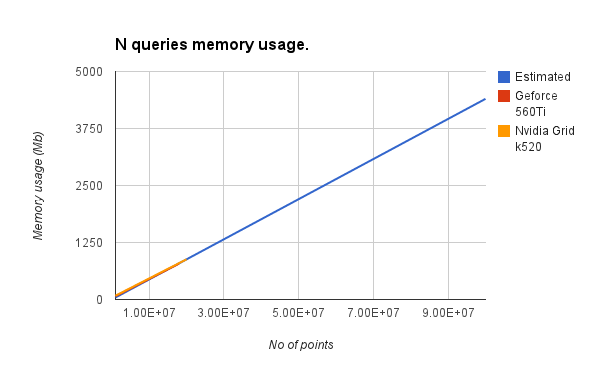
\includegraphics[width=120mm]{../gfx/memory-usage-kd-search.png}

\caption{Memory usage of kd-search.}
\label{fig:memory-usage-kd-search}
\end{figure}

Also in this case our estimation fit the real consumption with a high degree of accuracy.

Further work:
\begin{itemize}
    \item Look at memory optimization.
    \item Improve utiliti methods like: accumulateindex, minReduce.
    \item Forloop Unrolling.
\end{itemize}

% subsubsection parallel_improvements (end)

\subsubsection{V1.4 Release notes} % (fold)
\label{ssub:v14_release_notes}

Version 1.4 introduces the possibility of a variable k when searching. Testing the impact of varying the size of k was performed with a fixed number of 1000 repeated single queries. The timing results are shown in the following graph.

\begin{figure}[ht!]
\centering
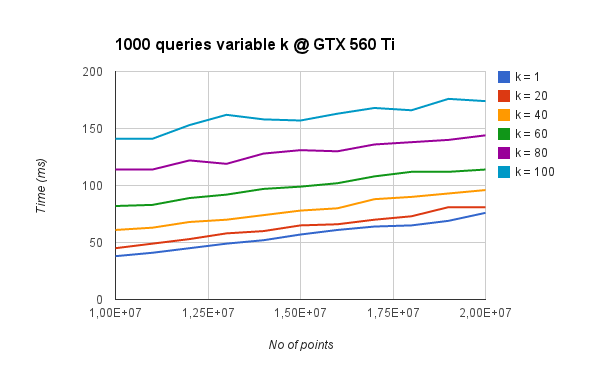
\includegraphics[width=120mm]{../gfx/v14_variable_k.png}

\caption{Variable k timing results.}
\label{fig:v14_variable_k}
\end{figure}

As expected, increasing k seems to increases the runtime with a constant factor. How this will affect searches in bigger trees and with a larger number of query-points should be explored next.

Timing tests of the build time and query time for n queries and k = 1 was performed on a GeForce GTX 560 and at Amazon Web Services (AWS). For the GTX card we get the following graph.

\begin{figure}[ht!]
\centering
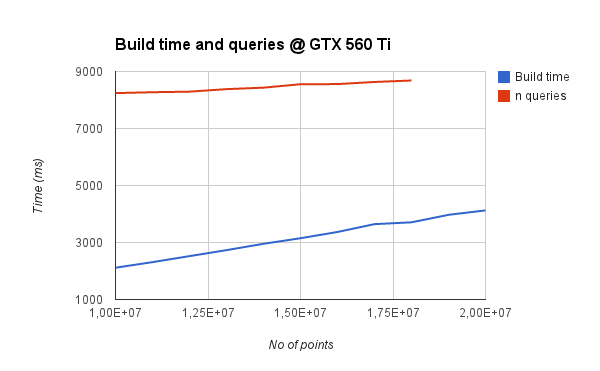
\includegraphics[width=120mm]{../gfx/v14_build_query_gtx.png}

\caption{Build and query times for v1.4.}
\label{fig:v14_build_query_gtx}
\end{figure}

Querying for n points still takes a lot of time, but the time increase related to the number of points seems to be lower than the build time. This trend is more prominent when we look at the results from our tests on AWS, graphed below.

\begin{figure}[ht!]
\centering
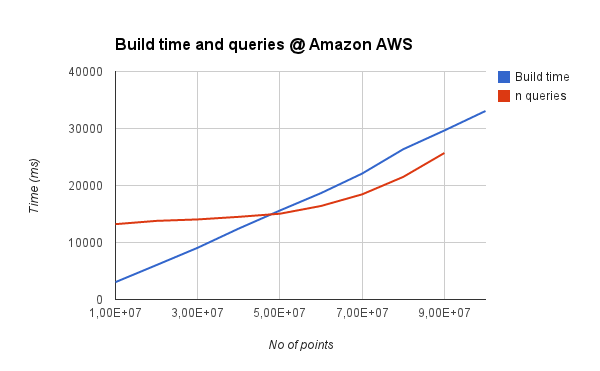
\includegraphics[width=120mm]{../gfx/v14_build_query_aws.png}

\caption{Build times and queries on AWS.}
\label{fig:v14_build_query_aws}
\end{figure}

Here we see that the runtime for the tree building algorithm catches up with the search time, and surpasses it around 50 million points. This is an interesting result.

From this graph we can see that on the AWS GPU, we are able, for 90 million points, to build the tree and query for the closest point, k = 1, in a total of ~30s + ~26s = ~56s < one minute.

Source data for all graphs can be found in
%[this spreadsheet](https://docs.google.com/spreadsheets/d/1I-qxnPa2FuYs7ePQC7d9v0GVHoYlr4CY6QdJbbNUlYo/edit?usp=sharing).

% subsubsection v14_release_notes (end)

\subsubsection{V1.3 Release notes} % (fold)
\label{ssub:v13_release_notes}

Version 1.3 introduces a couple of new features. Firstly the tree-building algorithm has been updated to also cache the location of the different children of each node in the tree. A small bug related to partition of the point-cloud list was also ironed out. This gives a tree building algorithm whit the following runtime results, comparable with the previous versions of this implementation:

\begin{figure}[ht!]
\centering
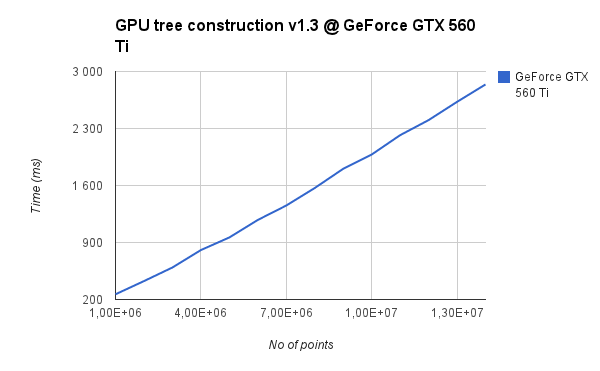
\includegraphics[width=120mm]{../gfx/construction_v13_gtx_560.png}

\caption{Construction timing results v13 @ gtx 560.}
\label{fig:construction_v13_gtx_560}
\end{figure}

After a surprising amount of fiddling, querying for a large number of query-points was finally parallelized in version 1.3. This gave improved performance when querying many times in the same point cloud. 14 million queries in a point cloud of 14 million points can now be done on average in ~8 seconds. Compared to the estimated ~17 seconds needed by the serial implementation.

\begin{figure}[ht!]
\centering
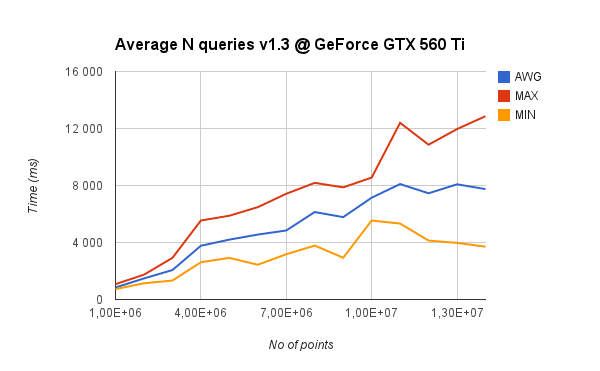
\includegraphics[width=120mm]{../gfx/n_queries_v13_gtx_560.png}

\caption{n queries timing results v13 @ gtx 560.}
\label{fig:n_queries_v13_gtx_560}
\end{figure}

Unfortunately, this early parallelization gave us quite unstable results. The data in the graph is based on ten timing runs, where the average, minimum and maximum values are collected in three series. As we can see, there is quite a big spread between the best and worst results. Looking at the raw data points for the ten series confirms that this is not a problem caused by a small number of outliers:

\begin{figure}[ht!]
\centering
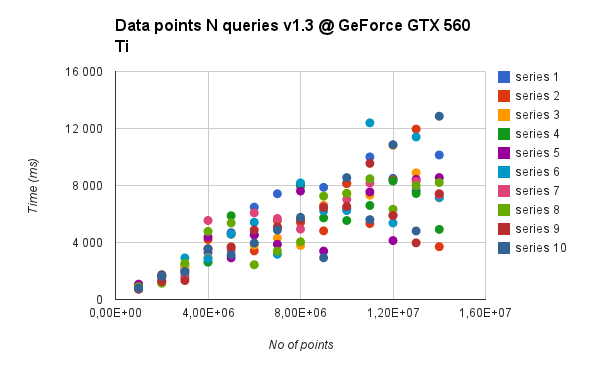
\includegraphics[width=120mm]{../gfx/scatter_n_queries_v13_gtx_560.png}

\caption{Scatter n queries timing results v13 2 gtx 560.}
\label{fig:scatter_n_queries_v13_gtx_560}
\end{figure}

Some instability would be expected, as the amount of pruning that can be achieved when searching for points in the kd-tree is dependent on the value you search for, but this amount of spread was unexpected. This behavior should be investigated further, as it seems to be indicating some kind of implementation error.

Combining the results from the search and the tree-building, gives the following runtime for a sequence of building and N queries:

\begin{figure}[ht!]
\centering
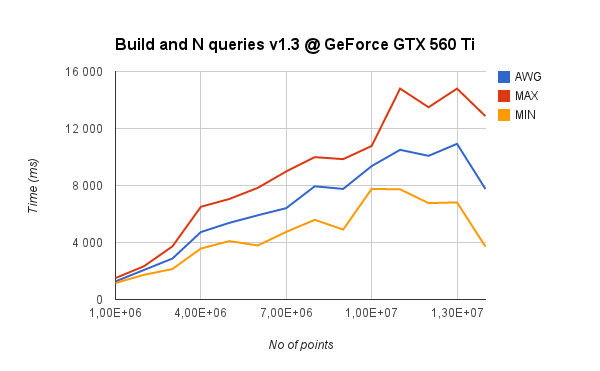
\includegraphics[width=120mm]{../gfx/constructionand_n_queries_v13_gtx_560.png}

\caption{Construction and n queries v13 @ gtx 560.}
\label{fig:constructionand_n_queries_v13_gtx_560}
\end{figure}
% subsubsection v13_release_notes (end)
% subsection kd_tree_based_effort (end)
